\chapter{Analýza}

Jelikož původní záměr zněl rozšířit mobilní aplikaci Catcher,
měli bychom se v této kapitole zabývat jejím průzkumem. Neopomene ani jiné podobné projekty.
V druhé části se podíváme na možnosti našeho řešení.

\section{Existující řešení}

\subsection*{Mobilní aplikace Catcher}

V roce 2013~\cite{cald_catcher} byla zveřejněna první verze této aplikace pro mobilní telefony s operačním systémem Android.
Autory jsou dva aktivní hráči Jiří Voseček a Ondřej Burkert. Aplikace si od svého vzniku získala velkou popularitu
ve~frisbee komunitě a dnes je používána na většině českých turnajů. Umí zadávat výsledky
zápasů včetně podrobného průběhu bodů, rozhodovat o umístění v základních skupinách, počítat statistiky hráčů,
odevzdávat a zveřejnit vzájemná hodnocení SOTG týmů na~turnaji. Dokáže omezeně importovat oficiální soupisky týmů
na nadcházející turnaje spadající pod Českou asociaci létajícího disku.

Kromě mobilní aplikace Catcher byl vytvořen backend v PHP~\cite{php}, který ukládá a počítá data na serveru. Ten však není
objektově orientovaný a~všechna jeho eventuální rozšíření jsou velmi náročná.

\subsubsection*{Výhody}
\begin{itemize}
  \item Backend je využíván webovou aplikací (frisbee.cz) a mobilní aplikací na~OS~Android.
  \item Přes webový prohlížeč lze přistupovat k emulátoru aplikace.
  \item Systém je již mezi organizátory turnajů zaběhnutý a na Google Play
    \footnote{Online distribuční služba, kde jsou k dispozici aplikace pro mobilní telefony a tablety s~OS Android.}
    má již více než 1000 stáhnutí~\cite{catcher_play}.
  \item Umí importovat soupisky na oficiální turnaje ČALD.
\end{itemize}

\begin{figure}[ht!]
\centering
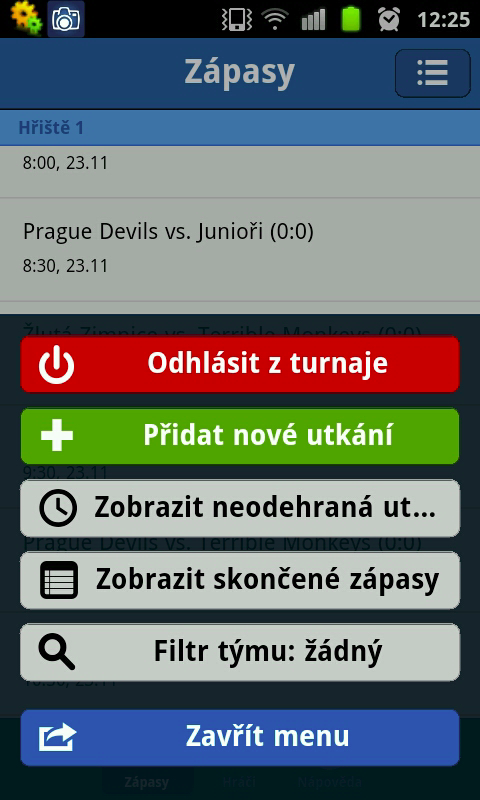
\includegraphics[width=60mm]{./images/catcher.png}
\caption{Mobilní aplikace Catcher~\cite{catcher_play}\label{overflow}}
\label{fig:uwsgi}
\end{figure}

\subsubsection*{Nevýhody}
\begin{itemize}
  \item Import soupisek z databáze ČALD je pouze poloautomatický. Administrátor musí před každým turnajem
    import spustit a zkontrolovat, zda se data uložila validně. Tomuto stavu nepřispívá ani fakt,
    že databáze ČALD, ze které se import provádí, je velmi špatně navržena.
  \item Nedisponuje žádným rozhraním, které by mohly používat další klientské aplikace.
  \item Automaticky nedoplňuje týmy v zápasech play-off do dalších kol (např.~vítěze semifinále do finále apod.).
  \item Při vytváření turnaje neprobíhá žádná kontrola validity dat.
    Lze tak vytvořit spoustu chybných utkání, které se pak musí opravovat. 
\end{itemize}

\subsection*{Ultimate Organizer}

Aplikace zveřejněná v roce 2004~\cite{ultimate_organizer}, napsaná v PHP a používaná na velkých akcích jako mistrovství světa nebo Evropy
pro sledování výsledků a statistik. Poskytuje tvorbu a správu turnajů, týmů, hráčů,
výsledků, rozpisů atd. Podporuje vícejazyčnost, tisk rozpisů v PDF, přístup pro mobilní telefony
a~spoustu dalších vlastností. Dokáže zobrazit podrobné detaily o průběhu zápasů.

\subsubsection*{Výhody}
\begin{itemize}
  \item Rozsáhlá aplikace poskytující nepřeberné množství možností.
  \item Aplikace má za sebou již více než 10 let fungování.
  \item Poskytuje přístup pro mobilní telefony s webovým prohlížečem.
\end{itemize}

\subsubsection*{Nevýhody}
\begin{itemize}
  \item Nefunguje jako webová aplikace. Uživatel si musí stáhnout zdrojové kódy a aplikaci si sám nasadit na svém počítači nebo serveru.
  \item Neposkytuje žádné rozumné rozhraní, tudíž pro ni nelze vytvořit žádného klienta.
  \item Nelze sledovat dlouhodobější statistiky napříč týmy a hráči. Všechny výsledky se týkají pouze jednoho konkrétního turnaje.
\end{itemize}

\subsection*{Ultimate Central}

Webová aplikace~\cite{ultimate_central}, která slouží především ke správě soupisek na~turnajích. Pořadatel turnaje vytvoří událost
v kalendáři a zapíše všechny účastnící se týmy. Ty pak musí odevzdat svoje soupisky a potvrdit náležité dokumenty,
které jsou na~některých turnajích povinností (např. zřeknutí se možnosti žalovat organizátora aj.).
Kromě toho dokáže ukládat výsledky zápasů a hodnocení SOTG. 

\begin{figure}[ht!]
\centering
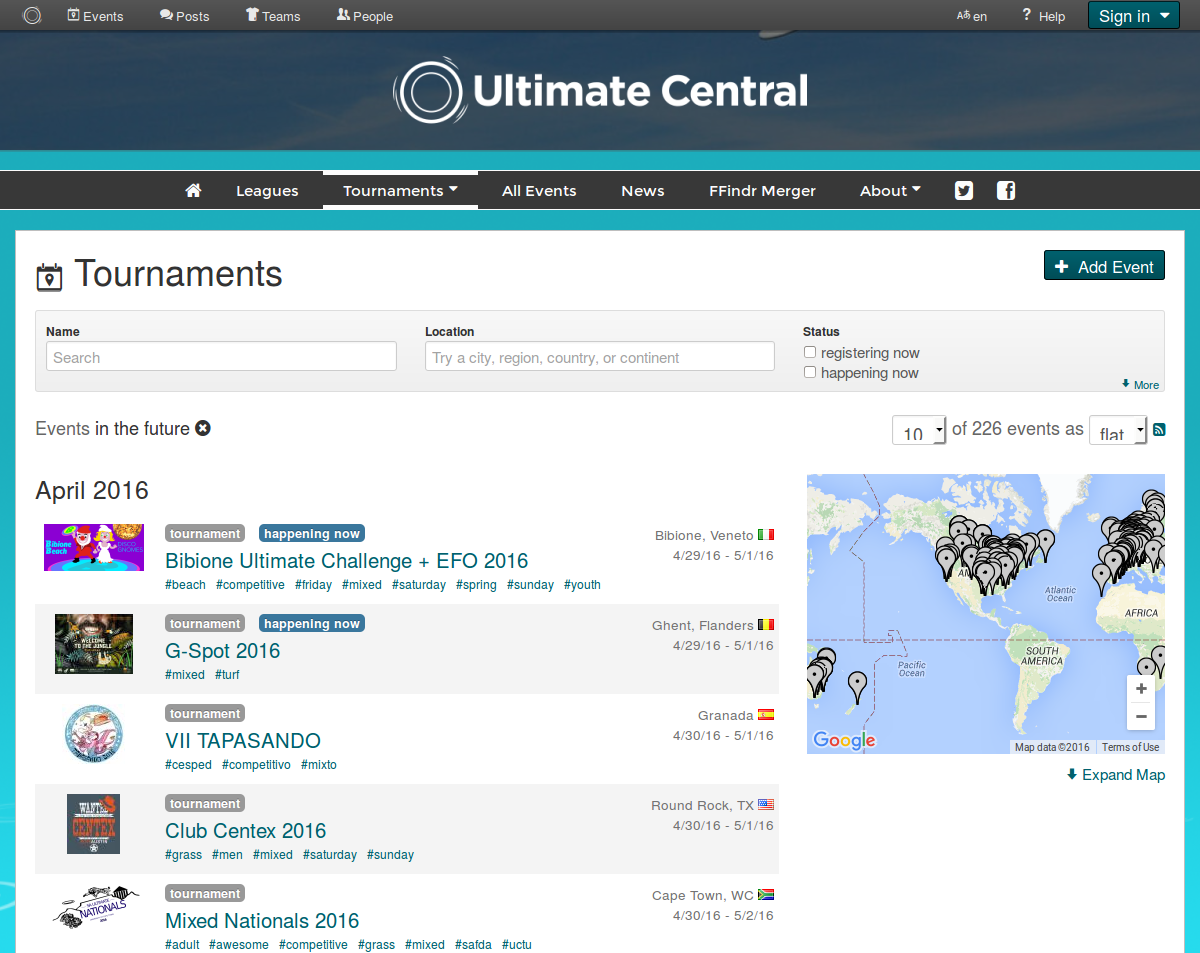
\includegraphics[width=130mm]{./images/ultimate-central.png}
\caption{Webová aplikace Ultimate Central\label{overflow}}
\end{figure}

\subsubsection*{Výhody}
\begin{itemize}
  \item Umožňuje vytvořit jednoduchou webovou stránku pro každý turnaj, na~které lze shrnout důležité informace pro všechny účastníky.
  \item Aplikace je dostupná ve webovém prohlížeči.
\end{itemize}

\subsubsection*{Nevýhody}
\begin{itemize}
  \item Neslouží ke statistikám. Do systému se zapisují pouze výsledky a hodnocení SOTG.
  \item Vyžaduje registraci a přihlašení každého jednotlivého hráče na turnaji.
  \item Stejně jako obě předchozí aplikace neposkytuje rozhraní, které by mohla využít například mobilní aplikace.
\end{itemize}

\subsection{Výsledek}

Průzkum existujících řešení naznačil, že náš projekt má smysl. Stále chybí aplikace,
která by byla zároveň plně automatizovaná (před započetím turnaje se vytvoří rozpis a~ten se
již doplňuje na základě zadaných výsledků), měla rozhraní pro libovolné tenké klienty
a~dokázala využít data z~databáze ČALD.

\section{Možnosti řešení}

Protože už od počátku známe požadavek na možnost připojení klienta v~podobě mobilní nebo webové aplikace,
je nutné poskytnout žadatelům o~přístup rozhraní, které dostatečně pokryje jejich požadavky.
Z úvodní kapitoly víme, že webová služba se dělí na dva typy - SOAP a REST.

\subsection{SOAP}

Protokol SOAP (\textit{Simple Object Access Protocol}) vystavuje aplikační logiku jako službu
a~je proveden v~syntaxi jazyka XML~\cite{xml}. Výhodou standartního značkovacího jazyka je jeho rozšíření
a značná podpora ve většině programovacích jazycích. Syntaxe XML je pro člověka relativně čitelná,
protože bývá zdlouhavá, avšak počítač musí parsování dat věnovat více času i paměti.

Nevýhodou je nestálost prostředí. Ve chvíli, kdy dojde v~SOAP API ke~změ\-ně, klient může přestat pracovat,
protože si nemusí umět poradit s odpovědí, přesněji s novou strukturou přijímaného XML souboru.
Podobně je potřeba upravovat při změnách API i strukturu požadavku.

% IDEA: Moznost napsat vice o SOAP, napriklad vlozit nejakou ukazku.
% SOAP služby standartně obsahují v URL nějaké sloveso (např. zobrazInfo).
 
\subsection{REST}

Protokol REST (\textit{Representational State Transfer}) je architektonický styl návrhu API popsaný Royem Fieldingem \cite{fielding}.
Je založený na vystavování a jednotném přístupu ke~zdrojům\footnote{resources}, kterými jsou určitá data.
Přistupuje se k~nim pomocí HTTP metod GET, POST, DELETE a PUT.

RESTová služba používá pro přenos dat řadu formátů, nejstandartnějšími jsou XML a JSON~\cite{json}.
JSON je datově méně náročnější a stejně jako XML je podporován v mnoha programovacích jazycích.

\subsubsection*{Zdroj}

Architektonický styl REST je postaven na základním prvku -- zdroji. Jde o~logický objekt,
který lze vyjádřit smysluplnou reprezentací, a~s~kterém lze manipulovat pomocí zpřístupněných metod.
Každý zdroj má svůj unikátní identifikátor URI\footnote{Uniform Resource Identifier}.

\subsubsection*{Požadavky na RESTové rozhraní}

Aby se mohlo nějaké aplikační rozhraní požadovat za RESTové (tzv. RESTful),
musí splňovat několik základních předpokladů definované Fieldingem \cite{fielding}.
Nyní si uvedeme ty nejdůležitější:

\begin{description}
    \item[Architektura klient-server]
    Rozděluje zodpovědnost mezi různé části. Klientské aplikace se nemusí starat o správu dat a server o jejich prezentaci.
    Z toho vyplývá možnost vyvíjet obě kompomenty (klient a server) nezávisle na sobě.
    \item[Bezstavovost]
    Aplikační stav je udržován na straně klienta. Všechny požadavky tak obsahují pouze informace nutné k jeho zpracování.  
    \item[Jednotné rozhraní]
    Pomocí unikátního identifikátoru lze získat reprezentaci nebo manipulovat s libovolným zdrojem.
    Klient musí být schopen s daným zdrojem manipulovat na základě jeho reprezentace. Zprávy by měly být dostatečně popisné.
\end{description}

\subsection{Shrnutí}

Z předcházejícího srovnání je patrné, že na flexibilní v budoucnu a rozšiřitelné rozhraní se spíše hodí REST.
Klienti nebudou tolik náchylní na úpravy API a~navíc jim bude možné data poskytnout ve~formátu JSON,
který se pro~jejich přenos hodí daleko více. XML je přece jenom spíše jazyk než formát dat.